\documentclass[14pt]{article}

\usepackage[utf8x]{inputenc}
\usepackage[russian]{babel}
\usepackage{graphicx}
\graphicspath{{images/}}
\DeclareGraphicsExtensions{.pdf,.png,.jpg}

\usepackage{amsmath}
\usepackage{pgfplots}

\usepackage{geometry} % Меняем поля страницы
\geometry{left=2cm}% левое поле
\geometry{right=1.5cm}% правое поле
\geometry{top=2cm}% верхнее поле
\geometry{bottom=2cm}% нижнее поле

\renewcommand{\theenumi}{\arabic{enumi}}
\renewcommand{\labelenumi}{\arabic{enumi}}
\renewcommand{\theenumii}{.\arabic{enumii}}
\renewcommand{\labelenumii}{\arabic{enumi}.\arabic{enumii}.}
\renewcommand{\theenumiii}{.\arabic{enumiii}}
\renewcommand{\labelenumiii}{\arabic{enumi}.\arabic{enumii}.\arabic{enumiii}.}

\begin{document}
\begin{titlepage}
	\begin{center}
		\fontsize{18pt}{20pt}\selectfont
		\textbf{Работа 3.6.1.}	
	
		\vspace{5cm}
		\fontsize{24pt}{25pt}\selectfont
		Спектральный анализ электрических сигналов. 
	\end{center}
	\begin{flushright}
		\fontsize{18pt}{20pt}\selectfont
		\vspace{14cm}
		\hspace{-3cm}
		\textit{Корнеев Е.С.}
	\end{flushright}		
\end{titlepage}

\begin{center}
	\fontsize{16pt}{18pt}\selectfont	
	Спектральный анализ электрических сигналов. 
\end{center}


\fontsize{14pt}{16pt}\selectfont
\vspace{1cm}
\textbf{Цель работы:} изучение спектрального состава периодических электрических сигналов.

\vspace{0.5cm}
\textbf{Оборудование:} анализатор спектра СК4-56, генератор прямоугольных импульсов Г5-54, генератор сигналов специальной формы Г6-34, осциллограф С1-76.

\vspace{1cm}

Многие физические процессы можно моделировать с помощью линейных дифференциальных уравнений. К решениям таких уравнений применим принцип суперпозиции: разнообразные сложные явления удобно представлять в виде суммы простых решений линейных уравнений. Для линейных уравнений такими простыми решениями являются гармонические функции. Математическая теория представления сложных функций в виде сумм гармонических составляющих получила название теории рядов и интегралов Фуръе.

В радиотехнике широко используется разложение сложных сигналов на гармонические колебания различных частот $\omega$. Функция $F(\omega)$‚ описывающая зависимость амплитуды гармоник от их частоты, называется \textsl{амплитудной спектральной характеристикой} - спектром исходного сигнала. Представление сложного периодического сигнала в виде суммы гармонических сигналов в математике называется разложением в ряд Фуръе. Непериодические сигналы представляются в виде интеграла Фурье.

Пусть заданная функция $f(t)$ периодически повторяется с частотой $\Omega_1 = 2\pi/T$, где $T$ - период повторения. Ее разложение в ряд Фурье имеет вид
\begin{equation}
f(t) = \frac{a_0}{2} + \sum_{i = 1}^{\infty}[a_n\cos(n\Omega_1t) + b_n\sin(n\Omega_2t)]
\end{equation}
или
\begin{equation}
f(t) = \frac{A_0}{2} + \sum_{i = 1}^{\infty}A_n\cos(n\Omega_1t - \psi_n).
\end{equation}
\noindent где $a_0/2 = A_0/2$ - среднее значение $f(t)$, $a_n$ и $b_n$ - амплитуды членов разложения, определяющиеся по формулам
$$
	a_n = \frac{2}{T}\int_{t_1}^{t_1 + T}f(t)\cos(n\Omega_1t)dt,
$$
$$
	b_n = \frac{2}{T}\int_{t_1}^{t_1 + T}f(t)\sin(n\Omega_1t)dt,
$$
\noindent точку $t_1$ можно выбрать произвольно. При этом между коэффициентами существует следующая связь:
$$
	A_n = \sqrt{a_n^2 + b_n^2};~~~\psi_n = \arctan\frac{b_n}{a_n}
$$
\noindent Таким образом, видно, что сигнал раскладывается в сумму сигналов с частотами $\Omega_1$, $2\Omega_1$, $3\Omega_1$, и т.д. Представляя $\cos\alpha$ в виде
$$
	\cos\alpha = \frac{e^{i\alpha} + e^{-i\alpha}}{2}
$$
\noindent и подставляя в (2):
$$
	f(t) = \frac{1}{2}\left(A_0 + \sum_{n = 1}^{\infty}A_ne^{-i\psi_n}e^{in\Omega_1t} + \sum_{n = 1}^{\infty}A_ne^{i\psi_n}e^{-in\Omega_1t}\right)
$$
\noindent Вводя комплексные амплитуды
\begin{equation}
\widetilde{A_n} = A_ne^{-i\psi_n};~~\widetilde{A_{-n}} = A_ne^{i\psi_n};~~\widetilde{A_0} = A_0
\end{equation}
\noindent получим
\begin{equation}
f(t) = \frac{1}{2}\sum_{n = -\infty}^{\infty}\widetilde{A_n}e^{in\Omega_1t}
\end{equation}

 
Видно, что введение отрицательных частот ($-n\Omega_1$) позволяет записать разложение Фурье простым способом. (3) обеспечивают действительность суммы (4): каждой частоте 
$k\Omega_1$ соответствует в (2) один член ($n = k$), а в (4) - два ($n = k$ и $n = -k$). Формулы (3) позволяют переходить от комплексного представления и обратно. 

Для рассчета комплексных амплитуд умножим левую и правую части (4) на $e^{-ik\Omega_1t}$ и проинтегрируем за период, например, от 0 до $2\pi/\Omega_1$. В правой части обнулятся все члены, кроме $n = k$, дающего $A_kT/2$. Поэтому
$$
	A_k = \frac{2}{T}\int_0^Tf(t)e^{-ik\Omega_1t}dt.
$$

Теперь рассмотрим функции, исследуемые в работе.

\vspace{1cm}
\textbf{Периодическая последовательность прямоугольных сигналов} с амплитудой $V_0$, длительностью $\tau$, частотой повторения $f_{\text{повт}} = 1/T$, где $T$ - период повторения импульсов. 

\begin{figure}[h!]
	\center{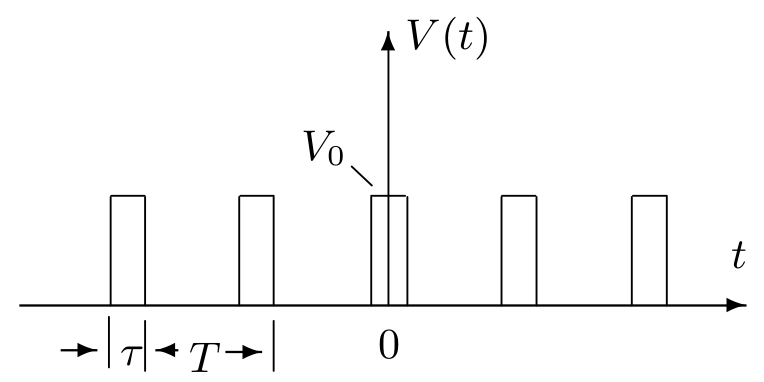
\includegraphics[width = 10cm]{1}}
	\caption{Периодическая последовательность прямоугольных импульсов}
	\label{fig:image}
\end{figure}

Найдем среднее значение:
$$
	\langle V\rangle = \frac{a_0}{2} = \frac{A_0}{2} = \frac{1}{T}\int_{-\tau/2}^{\tau/2}V_0dt = V_0\frac{\tau}{T}
$$

Амплитуды косинусных составляющих будут равны
$$
	a_n = \frac{2}{T}\int_{-\tau/2}^{\tau/2}V_0\cos(n\Omega_1t)dt = 2V_0\frac{\tau}{T}\frac{\sin(n\Omega_1\tau/2)}{n\Omega_1\tau/2} \sim \frac{\sin(x)}{x}
$$

\begin{figure}[h!]
	\center{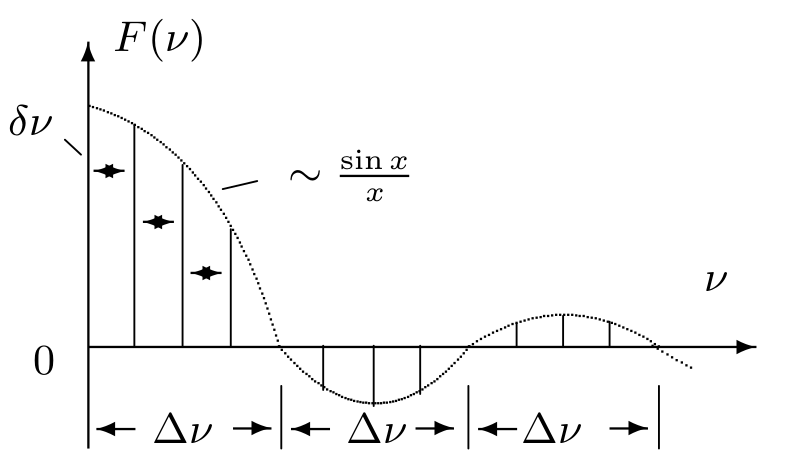
\includegraphics[width = 10cm]{2}}
	\caption{Спектр периодической последовательности прямоугольных импульсов}
	\label{fig:image}
\end{figure}

Поскольку функция четная, все амплитуды синусоидальных гармоник будут нулевыми. Амплитуды гармоник меняются по закону $\frac{\sin(x)}{x}$. На графике изображен случай, когда $T$ крастно $\tau$. Назовем шириной спектра $\Delta\nu$ расстояние от первого максимума, возникающего от главного максимума до первого нуля, возникающего при 
$\Omega_1 = 2\pi/T$. При этом $\Delta\omega\tau \approx 2\pi$, или $\Delta\nu\Delta t \approx 1$.

\vspace{1cm}
\textbf{Периодическая последовательность цугов} гармонического колебания $V_0\cos(\omega_0t)$ с длительностью цуга $\tau$ и периодом повторения $T$. 

\begin{figure}[h!]
	\center{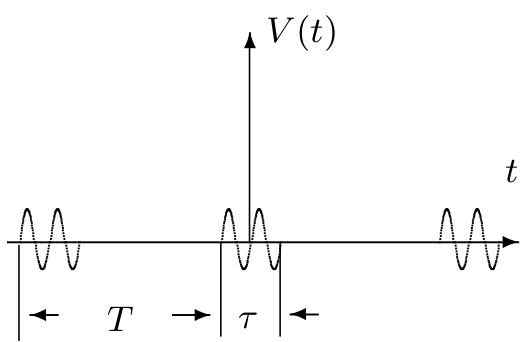
\includegraphics[width = 10cm]{3}}
	\caption{Периодическая последовательность цугов}
	\label{fig:image}
\end{figure}

Функция также симметричная относительно $t = 0$. Амплитуда $n-$й гармоники определяется выражением
$$
	A_n = a_n = \frac{2}{T}\int_{-\tau/2}^{\tau/2}V_0\cos(\omega_0t)\cdot\cos(n\Omega_1t)dt = 
$$
$$
	= V_0\frac{\tau}{T}\left(\frac{\sin[(\omega_0 - n\Omega_1)\frac{\tau}{2}]}{(\omega_0 - n\Omega_1)\frac{\tau}{2}} + 
	                         \frac{\sin[(\omega_0 + n\Omega_1)\frac{\tau}{2}]}{(\omega_0 + n\Omega_1)\frac{\tau}{2}}
	                   \right)
$$

\begin{figure}[h!]
	\center{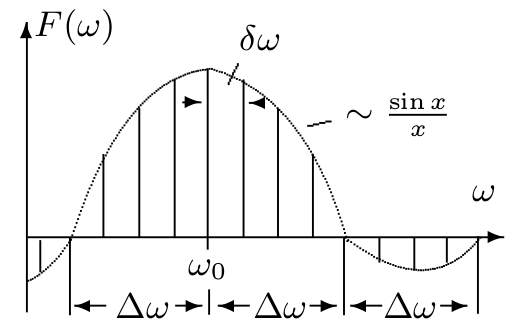
\includegraphics[width = 10cm]{4}}
	\caption{Спектр периодической последовательности цугов}
	\label{fig:image}
\end{figure}

Такое спектральное распределение $F(\omega)$ для случая, когда $T$ кратно $\tau$, представлено на рис. 5. Сравнивая этот график с аналогичным для прямоугольных импульсов, видим, что они аналогичны, но максимумы сдвинуты на почастоте на $\omega_0$. 

\vspace{1cm}
\textbf{Амплитудно-модулированные сигналы}. Рассмотрим гармонические колебания частоты $\omega_0$, амплитуда которых медленно меняется по гармоническому закону с частотой 
$\Omega$ ($\Omega \ll \omega_0$):
\begin{equation}
f(t) = A_0[1 + m\cos(\Omega t)]\cos(\omega t)
\end{equation}

\begin{figure}[h!]
	\center{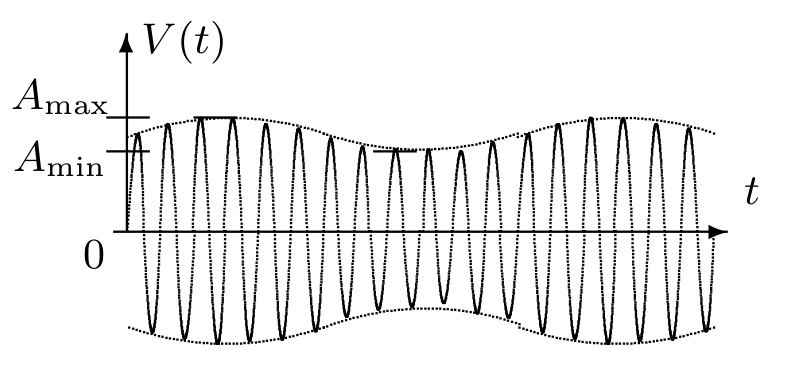
\includegraphics[width = 10cm]{5}}
	\caption{Гармонические колебания, модулированные по амплитуде}
	\label{fig:image}
\end{figure}

Коэффициент $m$ называется глубиной модуляции. При $m < 1$ амплитуда колебаний меняется от минимальной $A_{min} = A_0(1 - m)$ до максимальной $A_{max} = A_0(1 + m)$. Глубина модуляции может быть представлена в виде 
$$
	m = \frac{A_{max} - A_{min}}{A_{max} + A_{min}}
$$

Преобразовывая уравнение (5), получим спектр:
$$
	f(t) = A_0\cos(\omega_0t) + A_0m\cos(\Omega t)\cos(\omega_0t) = 
$$
$$
	= A_0\cos(\omega_0t) + \frac{A_0m}{2}\cos(\omega + \Omega)t + \frac{A_0m}{2}\cos(\omega - \Omega)t
$$

\begin{figure}[h!]
	\center{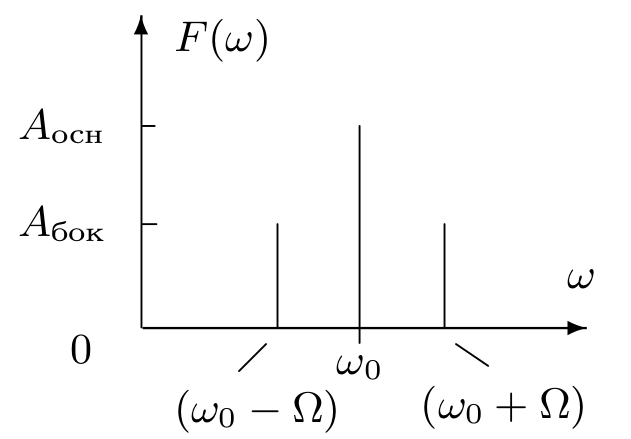
\includegraphics[width = 10cm]{6}}
	\caption{Спектр гармонических колебания, модулированных по амплитуде}
	\label{fig:image}
\end{figure}

Спектр $F(\omega)$ таких колебаний содержит три составляющих. Основная компонента представляет собой исходное немодулированное колебание с несущей частотой $\omega_0$ и амплитудой $A_{\text{осн}} = A_0$ - первое слагаемое в правой части последнего уравнения. Боковые компоненты спектра соответствуют гармоническим колебаниям с частотами 
($\omega_0 + \Omega$) и ($\omega_0 - \Omega$) - второе и третье слагаемые. Амлитуды этих колебаний одинаковы и составляют $m/2$ от амплитуды немодулированного сигнала:
$A_{\text{бок}} = A_0m/2$.

\newpage
\textbf{А. Исследование спектра периодической последовательности прямоугольных импульсов}

\textbf{Экспериментальная установка.} 

Схема для исследования спектра периодической последовательности прямоугольных импульсов представлена на рис. 7. Сигнал с выхода генератора прямоугольных импульсов Г5-54 подаётся на вход анализатора спектра и одновременно - на вход У осциллографа. С генератора импульсов на осциллограф подаётся также сигнал синхронизации, запускающий ждущую развёртку осциллографа. При этом на экране осциллографа можно наблюдать саму последовательность прямоугольных импульсов, а на экране ЭЛТ анализатора спектра - распределение амплитуд спектральных составляющих этой последовательности.

В наблюдаемом спектре отсутствует информация об амплитуде нулевой гармоники, т. е. о величине постоянной составляющей; её местоположение (начало отсчёта шкалы частот) отмечено небольшим вертикальным выбросом.

\begin{figure}[h!]
	\center{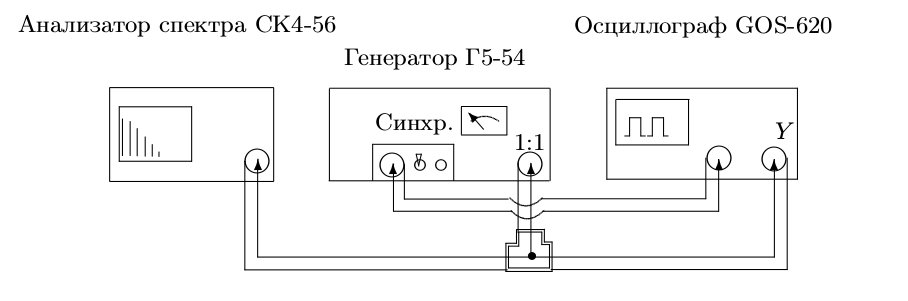
\includegraphics[width = 16cm]{fac1}}
	\caption{Схема для исследования периодической последовательности приямоугольных импульсов}
	\label{fig:image}
\end{figure}


\newpage
\textbf{Б. Исследование спектра периодической последовательности цугов гармонических колебаний}

\textbf{Экспериментальная установка.} 

Исследование спектра периодически чередующихся цугов гармонических колебаний проводится по схеме, изображённой на рис. 8. Генератор Гб-З4 вырабатывает синусоидальные колебания высокой частоты. На вход АМ (амплитудная модуляция) генератора Гб-З4 подаются прямоугольные импульсы с генератора Г5-54 и синусоида модулируется - «нарезается» на отдельные куски - цуги. Эти цуги с выхода генератора Гб-З4 поступают на вход спектроанализатора и одновременно на вход У осциллографа. Сигнал синхронизации подаётся на вход Х осциллографа с генератора импульсов.

\begin{figure}[h!]
	\center{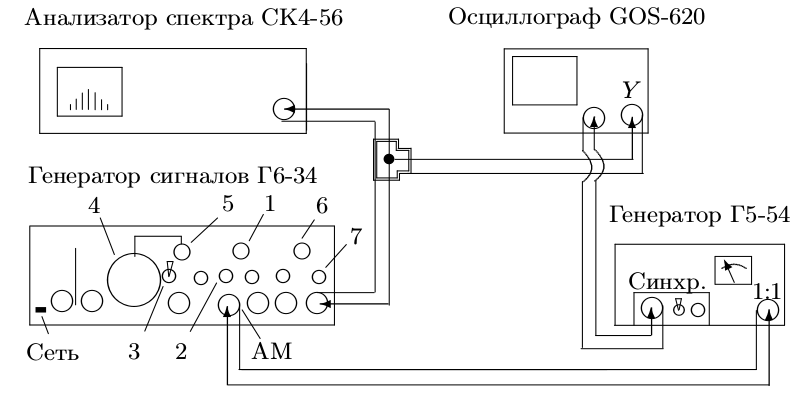
\includegraphics[width = 14cm]{fac2}}
	\caption{Схема для исследования периодической последовательности цугов высокочастотных колебаний}
	\label{fig:image}
\end{figure}


\newpage
\textbf{В. Исследование спектра гармонических колебаний, модулированных по амплитуде}

\textbf{Экспериментальная установка.} 

Схема для исследования амплитудно-модулированного сигнала представлена на рис. 9. Модуляционный генератор встроен в левую часть генератора сигналов Гб-З4. Синусоидальный сигнал с частотой модуляции $f_{\text{мод}} = 1$ кГц подаётся с модуляционного генератора на вход АМ (амплитудная модуляция) генератора, вырабатывающего синусоидальный сигнал высокой частоты (частота несущей $\nu_0 = 25$ кГц). Амплитудно-модулированный сигнал с основного выхода генератора поступает на осциллограф и на анализатор спектра.

\begin{figure}[h!]
	\center{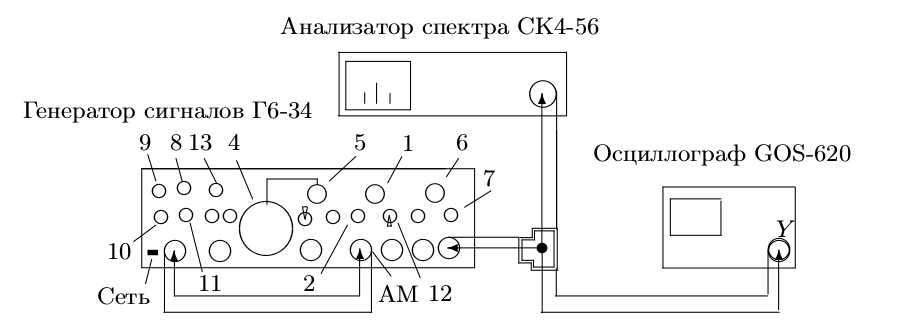
\includegraphics[width = 16cm]{fac3}}
	\caption{Схема для исследования спектра высокочастотного гармонического сигнала, промодулированного по амплитуде низкочастотным гармоническим сигналом}
	\label{fig:image}
\end{figure}




\end{document}